\documentclass[11pt]{article}
\usepackage[scaled=0.92]{helvet}
\usepackage{geometry}
\geometry{letterpaper,tmargin=1in,bmargin=1in,lmargin=1in,rmargin=1in}
\usepackage[parfill]{parskip} % Activate to begin paragraphs with an empty line rather than an indent %\usepackage{graphicx}
\usepackage{amsmath,amssymb, mathrsfs,  mathtools, dsfont}
\usepackage{tabularx}
\usepackage{tikz-cd}
\usepackage[font=footnotesize,labelfont=bf]{caption}
\usepackage{graphicx}
\usepackage{xcolor}
%\usepackage[linkbordercolor ={1 1 1} ]{hyperref}
%\usepackage[sf]{titlesec}
\usepackage{natbib}
\usepackage{../../Tianpei_Report}

%\usepackage{appendix}
%\usepackage{algorithm}
%\usepackage{algorithmic}

%\renewcommand{\algorithmicrequire}{\textbf{Input:}}
%\renewcommand{\algorithmicensure}{\textbf{Output:}}



\begin{document}
\title{Lecture 17: The Levi-Civita Connection}
\author{ Tianpei Xie}
\date{Nov. 4th., 2022}
\maketitle
\tableofcontents
\newpage
\section{The Tangential Connection Revisited}
\begin{itemize}
\item Suppose $\gamma: I \rightarrow M \subseteq \bR^n$ is a smooth curve. Then $\gamma$ can be regarded as either a smooth curve in $M$ or a smooth curve in $\bR^n$, and \emph{\textbf{a smooth vector field $V$ along $\gamma$}} that takes its values in $TM$ can be regarded as either a vector field along $\gamma$ in $M$ or a vector field along $\gamma$ in $\bR^n$. Let $\bar{D}_t(V)$ denote \emph{the covariant derivative of $V$ along $\gamma$} (\emph{\textbf{as a curve in $\bR^n$}}) with respect to \emph{\textbf{the Euclidean connection}} $\bar{\nabla}$, and let $D^{\top}_t(V)$ denote its covariant derivative along $\gamma$ (\emph{\textbf{as a curve in $M$}}) with respect to \emph{\textbf{the tangential connection}} $\nabla^{\top}$. 
\begin{align*}
\nabla^{\top}_{X}Y &= \pi^{\top}\paren{\bar{\nabla}_{\widetilde{X}}\widetilde{Y}}
\end{align*} where $X,Y \in \frX(M)$ and $\widetilde{X}, \widetilde{Y}$ are smooth extension of $X, Y$ to a neighborhood of $M$. 

\item Then we have the following proposition
\begin{proposition}
Let $M \subseteq \bR^n$ be an embedded submanifold, $\gamma: I \rightarrow M$ a smooth curve in $M$ , and $V$ a smooth vector field along  $\gamma$ that takes its values in $TM$ . Then for each $t \in I$,
\begin{align*}
D^{\top}_t(V(t)) &= \pi^{\top}\paren{\bar{D}_t(V(t))}.
\end{align*}
\end{proposition}

\item \begin{corollary}
Suppose $M \subseteq \bR^n$ is an embedded submanifold. A smooth curve $\gamma: I \rightarrow M$  is a \textbf{geodesic} with respect to the \textbf{tangential connection} on $M$ if and only if its \textbf{ordinary acceleration} $\gamma''(t)$ is \textbf{orthogonal} to $T_{\gamma(t)}M$ for all $t \in I$.
\end{corollary}

\item \begin{remark}
Let $(\bR^{r,s}, \bar{q}^{r,s})$ be the \emph{pseudo-Euclidean space of signature $(r,s)$}. If $M \subseteq \bR^{r,s}$ is an \emph{embedded Riemannian or pseudo-Riemannian submanifold}, then for each $p \in M$, the tangent space $T_{p}\bR^{r,s}$ decomposes as a \emph{\textbf{direct sum}} $T_{p}M \oplus N_{p}M$, where
$N_{p}M =(T_{p}M)^{\bot}$ is the \emph{orthogonal complement} of $T_{p}M$ with respect to $\bar{q}^{r,s}$. We let $\pi^{\top}: T_{p}\bR^{r,s} \rightarrow T_{p}M$ be the \emph{$\bar{q}^{r,s}$-orthogonal projection}, and define \emph{\textbf{the tangential connection}} $\nabla^{\top}$ on $M$ by
\begin{align*}
\nabla^{\top}_{X}Y &= \pi^{\top}\paren{\bar{\nabla}_{\widetilde{X}}\widetilde{Y}}
\end{align*},
where $\widetilde{X}, \widetilde{Y}$ are smooth extensions of $X$ and $Y$ to a neighborhood of $M$, and $\bar{\nabla}$ is the ordinary Euclidean connection on $\bR^{r,s}$. This is a well-defined connection on $M$.
\end{remark}
\end{itemize}
\section{Connections on Abstract Riemannian Manifolds}
\subsection{Metric Connections}
\begin{itemize}
\item \begin{remark}
For Euclidean connection, we have the following equation from the product rule
\begin{align*}
Z(\inn{X}{Y}) = \bar{\nabla}_{Z}\inn{X}{Y} &= \inn{\bar{\nabla}_{Z}X}{Y} + \inn{X}{\bar{\nabla}_{Z}Y}, \quad \forall X, Y, Z \in \frX(\bR^n).
\end{align*} It can be verified easily by computing in terms of the standard basis. For $X = X^i \partdiff{}{x^i}$, $Y = Y^i \partdiff{}{x^i}$ and $Z = Z^i \partdiff{}{x^i}$
\begin{align*}
\inn{X}{Y} &= \sum_{j=1}^{n}X^j\,Y^j \\
\text{LHS }&= Z\paren{\inn{X}{Y}} = Z^i\partdiff{}{x^i}\paren{\sum_{j=1}^{n}X^j,Y^j} \\
&= \sum_{j=1}^{n}Z^i\partdiff{X^j}{x^i}Y^j +  \sum_{j=1}^{n}Z^i\partdiff{Y_j}{x^i}X^{j}\\
\text{RHS }&= \inn{Z(X^j) \partdiff{}{x^j}}{Y} + \inn{X}{Z(Y^j) \partdiff{}{x^j}}\\
&=  \inn{Z^i\partdiff{X^j}{x^i} \partdiff{}{x^j}}{Y} + \inn{X}{Z^i\partdiff{Y_j}{x^i}\partdiff{}{x^j}}\\
&= \sum_{j=1}^{n}Z^i\partdiff{X^j}{x^i}Y^j + \sum_{j=1}^{n}Z^i\partdiff{Y_j}{x^i}X^{j}\\
\Rightarrow \text{LHS }&= \text{RHS } \qed
\end{align*}
\end{remark}

\item \begin{definition}
Let $g$ be a \emph{Riemannian or pseudo-Riemannian metric} on a smooth manifold $M$ (with or without boundary). A connection $\nabla$ on $TM$ is said to be \underline{\emph{\textbf{compatible with g}}}, or to be \underline{\emph{\textbf{a metric connection}}}, if it satisfies the following \emph{product rule} for all
$X, Y, Z \in \frX(M)$:
\begin{align}
 \conn{Z}{\inn{X}{Y}} &= \inn{\conn{Z}{X}}{Y} + \inn{X}{\conn{Z}{Y}} \label{eqn: metric_connection} \\
\Leftrightarrow Z\inn{X}{Y} &= \inn{\conn{Z}{X}}{Y} + \inn{X}{\conn{Z}{Y}} \nonumber
\end{align} 
\end{definition}



\item \begin{remark} More understanding of the equation \eqref{eqn: metric_connection}:
\begin{enumerate}
\item $\conn{Z}{\inn{X}{Y}} = \conn{Z}{(g(X, Y))}$. Note that $\inn{X}{Y} = g(X, Y) \in \cC^{\infty}(M)$ is \emph{a smooth function} since $g$ is a \emph{\textbf{covariant $2$-tensor}}.  Thus $\conn{Z}{\inn{X}{Y}} = Z\inn{X}{Y} \in \cC^{\infty}(M)$ since for $f \in \cC^{\infty}(M)$, the directional derivative of $f$ along direction of $Z$, $\conn{Z}{f} = Zf$. Intuitively, it measures \emph{\textbf{the directional derivatives of the angle} between two vector fields $X$ and $Y$ along the direction of vector field $Z$}.

\item $\inn{\conn{Z}{X}}{Y} = g\paren{\conn{Z}{X}, Y} \in \cC^{\infty}(M)$ measures \emph{\textbf{the angle between $\conn{Z}{X}$ and $Y$}}; similarly, $\inn{X}{\conn{Z}{Y}} = g\paren{X, \conn{Z}{Y}}$ measures \emph{\textbf{the angle between $X$ and $\conn{Z}{Y}$}}. In both terms,  $\conn{Z}{X}$ is the \emph{\textbf{directional derivative}} $X$ along $Z$, which is \emph{the difference} between $X$ and \emph{its infinitesimal parallel transport} along $Z$. 

\item The equation \eqref{eqn: metric_connection} states that  ``\emph{\textbf{the directional derivatives of the angle} between two vector fields $X$ and $Y$ along the direction of vector field $Z$} \emph{\textbf{is equal to}} the \emph{\textbf{sum of angles}} of \emph{the \textbf{directional derivative of one vector field} along direction of $Z$} \emph{\textbf{with respect to the other vector field}}".
\end{enumerate}
\end{remark}

\begin{figure}
\begin{minipage}[htb]{1\linewidth}
  \centering
  \centerline{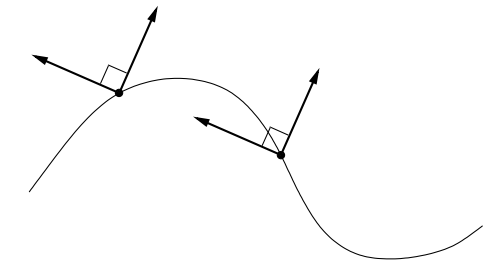
\includegraphics[scale = 0.5]{parallel_orthonormal_frame.png}}
\end{minipage}
\caption{\footnotesize{\textbf{A parallel orthonormal frame \citep{lee2018introduction}}}}
\label{fig: parallel_orthonormal_frame}
\end{figure}

\item \begin{proposition} (\textbf{Characterizations of Metric Connections}).\\
Let $(M, g)$ be a Riemannian or pseudo-Riemannian manifold (with or without boundary), and let $\nabla$ be a connection on $TM$. The following conditions are \textbf{equivalent}:
\begin{enumerate}
\item $\nabla$ is \textbf{compatible} with $g$: $\conn{Z}{\inn{X}{Y}} = \inn{\conn{Z}{X}}{Y} + \inn{X}{\conn{Z}{Y}}$.
\item $g$ is \textbf{parallel with respect to} $\nabla$: $\nabla g \equiv 0$.
\item In terms of any smooth local frame $(E_i)$, the \textbf{connection coefficients} of $\nabla$ satisfy
\begin{align}
\Gamma_{k,i}^{l}g_{l,j} + \Gamma_{k,j}^{l}g_{i,l} &= E_k(g_{i,j}).  \label{eqn: metric_connection_christoffel_symbol}
\end{align}
\item If $V, W$ are smooth vector fields along any smooth curve $\gamma$, then
\begin{align}
\frac{d}{dt}\inn{V}{W} &= \inn{D_tV}{W} + \inn{V}{D_tW}. \label{eqn: metric_connection_derivative_of_inn}
\end{align}
\item If $V, W$ are \textbf{parallel} vector fields \textbf{along a smooth curve} $\gamma$ in $M$, then $\inn{V}{W}$ is \textbf{constant} along $\gamma$.
\item Given any smooth curve $\gamma$ in $M$, every \textbf{parallel transport map} along $\gamma$ is a \textbf{linear isometry}.
\item  Given any smooth curve $\gamma$ in $M$, every \textbf{orthonormal basis} at a point of $\gamma$ can be \textbf{extended} to a \textbf{parallel orthonormal frame} along $\gamma$ (Fig. \ref{fig: parallel_orthonormal_frame})
\end{enumerate}
\end{proposition}

\item \begin{remark}
From the proposition statement 5,6,7 above, we see that \emph{\textbf{the metric connection}} $\nabla$ that is compatible with $g$ \emph{defines} \emph{the \textbf{parallel transport operation}} that maintains \emph{the \textbf{angle} between two vector fields \textbf{unchanged}}. In other word, \emph{\textbf{\underline{the parallel transport} defined by \underline{the metric connection}}} is  an \emph{\textbf{\underline{isometry}}} on the manifold. 
\end{remark}

\item \begin{corollary}
Suppose $(M, g)$ is a Riemannian or pseudo-Riemannian manifold with or without boundary, $\nabla$ is a \textbf{metric connection} on $M$, and $\gamma: I \rightarrow M$ is a smooth curve.
\begin{enumerate}
\item $\abs{\gamma'(t)}$ is \textbf{constant} if and only if $D_t\gamma'(t)$ is \textbf{orthogonal} to $\gamma'(t)$ for all $t \in I$.
\item If $\gamma$ is a \textbf{geodesic}, then $\abs{\gamma'(t)}$ is \textbf{constant}.
\end{enumerate}
\end{corollary}

\item \begin{proposition}
If $M$ is an embedded Riemannian or pseudo-Riemannian \textbf{submanifold} of $\bR^n$ or $\bR^{r,s}$, the \textbf{tangential connection} on $M$ is \textbf{compatible} with the \textbf{induced} Riemannian or pseudo-Riemannian \textbf{metric}.
\end{proposition}
\end{itemize}
\subsection{Symmetric Connections}
\begin{itemize}
\item \begin{remark}
For $X = X^i \partdiff{}{x^i}$, $Y = Y^i \partdiff{}{x^i}$, the Lie bracket between $X$ and $Y$ is
\begin{align*}
[X, Y] &= X(Y^i)\partdiff{}{x^i} - Y(X^i)\partdiff{}{x^i} \\
\text{since }\bar{\nabla}_{X}Y &= X(Y^i)\partdiff{}{x^i}, \\
\bar{\nabla}_{Y}X &= Y(X^i)\partdiff{}{x^i} \\
\Rightarrow [X, Y]  &=  \bar{\nabla}_{X}Y - \bar{\nabla}_{Y}X
\end{align*}
\end{remark}

\item \begin{definition}
A \emph{\textbf{connection}} $\nabla$ on the tangent bundle of a smooth manifold $M$ is \underline{\emph{\textbf{symmetric}}} if
\begin{align*}
\conn{X}{Y} - \conn{Y}{X} &= [X, Y]  \quad \text{for all }X,Y \in \frX(M),
\end{align*} where $[X, Y]$ is the Lie bracket of two vector fields.
\end{definition}

\item \begin{definition}
The \emph{\textbf{torsion tensor}} of the \emph{connection} $\nabla$ is a \emph{\textbf{smooth $(1,2)$-tensor field}} $\tau: \frX(M) \times \frX(M) \rightarrow \frX(M)$ defined by
\begin{align*}
\tau(X, Y) &:= \conn{X}{Y} - \conn{Y}{X} - [X, Y].
\end{align*}
\end{definition}

\item \begin{remark}
Thus, a connection $\nabla$ is \emph{\textbf{symmetric}} if and only if its torsion \emph{\textbf{vanishes}} identically $\tau \equiv 0$.
\end{remark}

\item \begin{remark} (\emph{\textbf{Coordinate Representation of Symmetric Connections}})\\
A connection is \emph{\textbf{symmetric}} if and only if \emph{its \textbf{connection coefficients}} in \emph{every coordinate frame} is \emph{\textbf{symmetric}} in \emph{\textbf{lower two indices}} That is, \underline{$\Gamma_{i,j}^{k} = \Gamma_{j,i}^{k}$} for all $i,j$. 
\end{remark}

\item \begin{proposition}
If $M$ is an embedded (pseudo-)Riemannian submanifold of a (pseudo-)Euclidean space, then the \textbf{tangential connection} on $M$ is \textbf{symmetric}.
\end{proposition}
\end{itemize}
\subsection{The Levi-Civita Connection}
\begin{itemize}
\item \begin{remark}
The last two propositions show that if we wish to single out a connection on each Riemannian or pseudo-Riemannian manifold in such a way that it matches the tangential connection when the manifold is presented as an embedded submanifold of $\bR^n$ or $\bR^{r,s}$ with the induced metric, then we must require at least that \emph{\textbf{the connection be compatible with the metric}} and \emph{\textbf{symmetric}}. 
\end{remark}

\item \begin{theorem} (\textbf{Fundamental Theorem of Riemannian Geometry}). \citep{lee2018introduction}\\
Let $(M, g)$ be a Riemannian or pseudo-Riemannian manifold (with or without boundary). There exists a \textbf{unique connection} $\nabla$ on $TM$ that \textbf{is compatible with $g$} and \textbf{symmetric}. It is called the \underline{\textbf{Levi-Civita connection of $g$}} (or also, when $g$ is \textbf{positive definite}, the \underline{\textbf{Riemannian connection}}).
\end{theorem}

\item \begin{corollary} (\textbf{Formulas for the Levi-Civita Connection}). \citep{lee2018introduction}\\
Let  $(M, g)$ be a Riemannian or pseudo-Riemannian manifold (with or without boundary), and let $\nabla$ be its \textbf{Levi-Civita connection}.
\begin{enumerate}
\item  \underline{(\textbf{In Terms of Vector Fields})}: If $X, Y, Z$ are smooth vector fields on $M$, then
\begin{align}
\inn{\conn{X}{Y}}{Z} &=\frac{1}{2}\paren{X\langle{Y,Z}\rangle + Y\langle{Z,X}\rangle - Z\langle{X,Y}\rangle -  \langle{Y, [X, Z]}\rangle - \langle{Z, [Y, X]}\rangle + \langle{X, [Z, Y]}\rangle}\label{eqn: levi_civita_formula_vector_fields}
\end{align}
(This is known as \underline{\textbf{Koszul's formula}}.)
\item \underline{(\textbf{In Coordinates})}: In any smooth coordinate chart for $M$, the \textbf{coefficients of the Levi-Civita connection} are given by
\begin{align}
\Gamma_{i,j}^{k} &= \frac{1}{2}g^{k,l}\paren{ \partdiff{}{x^i}g_{j,l} + \partdiff{}{x^j}g_{i,l} - \partdiff{}{x^l}g_{i,j} }.\label{eqn: levi_civita_formula_christoffel_symbol_metric}
\end{align}
\item (\textbf{In A Local Frame}): Let $(E_i)$ be a smooth \textbf{local frame} on an open subset $U \subseteq M$, and let $c_{i,j}^{k}: U \rightarrow \bR$ be the $n^3$ smooth functions defined by
\begin{align}
[E_i, E_j] &= c_{i,j}^k \, E_k\label{eqn: coefficient_lie_bracket}
\end{align}
Then \textbf{the coefficients of the Levi-Civita connection} in this frame are
\begin{align}
\Gamma_{i,j}^{k} &= \frac{1}{2}g^{k,l}\paren{E_i\,g_{j,l} + E_j\,g_{i,l} - E_l\,g_{i,j} - g_{j,m}c_{i,l}^{m} - g_{l,m}c_{j,i}^m + g_{i,m}c_{l,j}^m}. \label{eqn: levi_civita_formula_christoffel_symbol_local_frames}
\end{align}

\item (\textbf{In A Local Orthonormal Frame}): If $g$ is Riemannian, $(E_i)$ is a smooth \textbf{local orthonormal frame}, and the functions $c_{i,j}^k$ are defined by \eqref{eqn: coefficient_lie_bracket}, then
\begin{align}
\Gamma_{i,j}^{k} &= \frac{1}{2}\paren{ c_{i,j}^{k} - c_{i,k}^{j} - c_{j,k}^{i} } \label{eqn: levi_civita_formula_christoffel_symbol_ortho_local_frames}
\end{align}
\end{enumerate}
\end{corollary}

\item \begin{remark}
On every Riemannian or pseudo-Riemannian manifold, we will always use the Levi-Civita connection from now on without further comment.
\end{remark}

\item \begin{remark}
\emph{Geodesics} with respect to the Levi-Civita connection are called \underline{\emph{\textbf{Riemannian geodesics}}}, or
simply ``\emph{geodesics”} as long as there is no risk of confusion. 
\end{remark}

\item \begin{remark}
The \emph{\textbf{connection coefficients} $\Gamma_{i,j}^{k}$ of \textbf{the Levi-Civita connection}} in coordinates, given by \eqref{eqn: levi_civita_formula_christoffel_symbol_metric}, are called \underline{\emph{\textbf{the Christoffel symbols of $g$}}}.
\end{remark}

\item \begin{proposition}
\begin{enumerate}
\item The Levi-Civita connection on a (pseudo-)\textbf{Euclidean space} is equal to the \textbf{Euclidean connection}.
\item Suppose $M$ is an \textbf{embedded} (pseudo-)Riemannian \textbf{submanifold} of a (pseudo-)Euclidean space. Then the Levi-Civita connection on $M$ is equal to\textbf{ the tangential connection} $\nabla^{\top}$.
\end{enumerate}
\end{proposition}

\item \begin{proposition} (\textbf{Naturality of the Levi-Civita Connection}). \citep{lee2018introduction}\\
Suppose $(M,g)$ and $(\widetilde{M}, \widetilde{g})$ are Riemannian or pseudo-Riemannian manifolds with or without boundary, and let $\nabla$ denote the Levi-Civita connection of $g$ and $\widetilde{\nabla}$ that of $\widetilde{g}$. If $\varphi: M \rightarrow \widetilde{M}$ is an isometry, then $\varphi^{*}\widetilde{g} = \nabla$.
\end{proposition}

\begin{remark} 
An \emph{\textbf{isometry}} $\varphi$ between the manifold $M$ and $ \widetilde{M}$ can be used to define \emph{\textbf{the pullback connection}} in $M$ from \emph{the  Levi-Civita connection} $\widetilde{M}$. Recall that for general connections, we can only define a pullback connection if $\varphi$ is a \emph{diffeomorphism}.
\end{remark}

\item \begin{corollary} (\textbf{Naturality of Geodesics}). \\
Suppose $(M,g)$ and $(\widetilde{M}, \widetilde{g})$ are Riemannian or pseudo-Riemannian manifolds with or without boundary, and $\varphi: M \rightarrow \widetilde{M}$ is a \textbf{local isometry}. If $\gamma$ is a \textbf{geodesic} in $M$, then $\varphi \circ \gamma$ is a \textbf{geodesic} in $M$.
\end{corollary}

\begin{remark} 
An \emph{\textbf{isometry}} $\varphi$ between the manifold $M$ and $ \widetilde{M}$ maps a $\nabla$-geodesic in $M$ to a $\widetilde{\nabla}$ -geodesic in $\widetilde{M}$ for both \emph{Levi-Civita Connections} $\nabla$ and $\widetilde{\nabla}$.
\end{remark}

\item \begin{proposition}
Suppose $(M,g)$ is a Riemannian or pseudo-Riemannian manifold. The connection induced on each \textbf{tensor bundle} by the Levi-Civita connection is \textbf{compatible} with \textbf{the induced inner product on tensors}, in the sense that $X \inn{F}{G}= \inn{\conn{X}{F}}{G} + \inn{F}{\conn{X}{G}}$ for every vector field $X$ and every pair of smooth tensor fields $F, G \in T^{(k,l)}TM$.
\end{proposition}


\item \begin{proposition} (\textbf{Volume Preseving under Parallel Transport})\\
Let $(M, g)$ be an oriented Riemannian manifold. The Riemannian volume form of $g$ is \textbf{parallel} with respect to the Levi-Civita connection.
\end{proposition}

\item \begin{proposition} 
The \textbf{musical isomorphisms commute with the total covariant derivative operator}: if $F$ is any smooth tensor field with a \textbf{contravariant} $i$-th index
position, and $\flat$ represents the operation of lowering the $i$-th index, then
\begin{align}
\nabla (F^{\flat}) &= \paren{\nabla F}^{\flat}  \label{eqn: levi_civita_connection_flat_operation}
\end{align}
Similarly, if $G$ has a \textbf{covariant} $i$-th position and $\sharp$ denotes raising the $i$-th index, then
\begin{align}
\nabla (G^{\sharp}) &= \paren{\nabla G}^{\sharp}  \label{eqn: levi_civita_connection_sharp_operation}
\end{align}
\end{proposition}
\end{itemize}

\section{The Exponential Map}
\begin{itemize}
\item \begin{remark}
It is shown above that each initial point $p\in M$ and each initial velocity vector $v \in T_{p}M$ determine a \emph{\textbf{unique maximal geodesic}} $\gamma_v$. How do geodesics change if we vary the initial point or the initial velocity ?  The dependence of geodesics on the initial data is encoded in a map from the tangent
bundle into the manifold, called \emph{\textbf{the exponential map}}, whose properties are fundamental to the further study of Riemannian geometry. 
\end{remark}

\item \begin{lemma} (\textbf{Rescaling Lemma}).\\
 For every $p\in M$, $v \in T_{p}M$, and $c, t \in \bR$,
 \begin{align}
 \gamma_{c\,v}(t) = \gamma_{v}(c\,t) \label{eqn: exp_map_rescaling}
 \end{align} whenever either side is defined.
\end{lemma}

\item \begin{definition}
Define a subset $\cE \subseteq  TM$, \emph{\textbf{the domain of the exponential map}}, by
\begin{align*}
\cE = \set{v \in TM: \gamma_v\text{ is defined on an interval containing [0,1]}},
\end{align*}
and then define \underline{\emph{\textbf{the exponential map}}} $\exp: \cE \rightarrow M$ by
\begin{align*}
\exp(v)  &= \gamma_{v}(1)
\end{align*}
For each $p \in M$, the \emph{\textbf{restricted exponential map}} at $p$, denoted by $\exp_p$, is the restriction of $\exp$ to the set $\cE_p = \cE \cap T_{p}M$.
\end{definition}

\item \begin{remark}
The \emph{\textbf{exponential map} of a \textbf{Riemannian manifold}} should not be confused with \emph{the \textbf{exponential map} of a \textbf{Lie group}}. The two are closely related for \emph{\textbf{bi-invariant metrics}}, but in general they need not be. 
\end{remark}

\item \begin{remark}
Recall that a subset of a vector space $V$ is said to be \emph{\textbf{star-shaped}} \emph{with respect to a point} $x \in S$ if for every $y \in S$, the \emph{line segment} from $x$ to $y$ is contained in $S$.
\end{remark}

\item \begin{proposition}(\textbf{Properties of the Exponential Map}). \citep{lee2018introduction}\\
Let $(M, g)$ be a Riemannian or pseudo-Riemannian manifold, and let $\exp: \cE \rightarrow M$ be its exponential map.
\begin{enumerate}
\item  $\cE$ is an \textbf{open} subset of $TM$ containing the image of the \textbf{zero section}, and each
set $\cE_p \subseteq T_{p}M$ is \textbf{star-shaped with respect to $0$}.
\item For each $v \in TM$, the \textbf{geodesic} $\gamma_v$ is given by
\begin{align}
\gamma_{v}(t) &= \exp(v\,t) \label{eqn: exp_map_geodesic}
\end{align} for all $t$ such that either side is defined.
\item The exponential map is \textbf{smooth}.
\item For each point $p \in M$, the \textbf{differential} $d(\exp_p)_0: T_0(T_{p}M) \simeq T_{p}M \rightarrow T_{p}M$ is \textbf{the identity map} of $T_{p}M$, under the usual identification of $T_{0}(T_{p}M)$ with $T_{p}M$.
\end{enumerate}
\end{proposition}

\item \begin{remark} The \emph{\textbf{geodesic equation} under the initial boundary condition} can be written in the following form:
\begin{align}
\dot{x}^k(t) &= v^{k}(t) \\
\dot{v}^k(t) &= - v^{i}(t)v^j(t)\,\Gamma_{i,j}^{k}(x(t)) \label{eqn: geodesic_equation_first_order}
\end{align} Treating $(x^1 \xdotx{,} x^n, v^1 \xdotx{,} v^n)$ as coordinates on $U \times \bR^n$, we can recognize \eqref{eqn: geodesic_equation_first_order} as the equations for the \textbf{\emph{flow}} of \textbf{\emph{the vector field}} $G \in \frX(U \times \bR^n)$ given by
\begin{align}
G_{(x, v)} &= v^k\partdiff{}{x^k}\Bigr|_{(x, v)} - v^{i}v^j\,\Gamma_{i,j}^{k}(x)\partdiff{}{v^k}\Bigr|_{(x, v)}.
\end{align} The importance of $G$ stems from the fact that it actually defines \emph{\textbf{a global vector field on the total space of $TM$}}, called \underline{\emph{\textbf{the geodesic vector field}}}. It can be verified that the components of $G$ under a change of coordinates \emph{take the same form} in \emph{every coordinate chart}.

Note that $G$ acts on a function $f \in \cC^{\infty}(U \times \bR^n)$ as
\begin{align}
Gf(p, v) &= \frac{d}{dt}\Bigr|_{t=0}f(\gamma_v(t), \gamma_v'(t)). \label{eqn: geodesic_vector_field_act_function}
\end{align}
\end{remark}

\item \begin{proposition} (\textbf{Naturality of the Exponential Map}). \\
Suppose $(M, g)$ and $(\widetilde{M},\widetilde{g})$ are Riemannian or pseudo-Riemannian manifolds and $\varphi: M \rightarrow \widetilde{M}$ is a \textbf{local isometry}. Then for every $p \in M$, the following diagram commutes:
\[
  \begin{tikzcd}
    \cE_{p} \arrow{r}{d\varphi_p} \arrow[swap]{d}{\exp_p} & \widetilde{\cE}_{\varphi(p)} \arrow{d}{\exp_{\varphi(p)}} \\
    M \arrow{r}{\varphi} & \widetilde{M},
  \end{tikzcd}
\] where $\cE_p \subseteq T_{p}M$ and $ \widetilde{\cE}_{\varphi(p)} \subseteq T_{\varphi(p)}\widetilde{M}$ are the domains of the restricted exponential maps $\exp_p$ (with respect to $g$) and $\exp_{\varphi(p)}$ (with respect to $\tilde{g}$), respectively.
\end{proposition}

\item \begin{remark}
Under isometry transformation, the exponential map \emph{\textbf{remain unchanged}} from $TM$ to $T\widetilde{M}$.
\end{remark}

\item The following proposition shows that \emph{\textbf{local isometries}} of connected manifolds are \emph{\textbf{completely determined}} by their \emph{\textbf{values}} and \emph{\textbf{differentials}} at a single point.
\begin{proposition}
Let $(M, g)$ and $\widetilde{M},\widetilde{g})$ be Riemannian or pseudo-Riemannian manifolds, with $M$ \textbf{connected}. Suppose $\varphi, \psi: M \rightarrow \widetilde{M}$ are \textbf{local isometries} such that for some point $p \in M$, we have $\varphi(p) = \psi(p)$ and $d\varphi_p = d\psi_p$. Then $\varphi \equiv \psi$.
\end{proposition}

\item \begin{definition}
A Riemannian or pseudo-Riemannian manifold  $(M, g)$ is said to be \emph{\textbf{geodesically complete}} if \emph{every maximal geodesic} is defined for \emph{\textbf{all}} $t \in \bR$, or equivalently if \emph{the domain of the exponential map is all of $TM$}. 
\end{definition}
\end{itemize}

\section{Normal Neighborhoods and Normal Coordinates}
\begin{itemize}
\item \begin{definition}
Let $(M, g)$ be a Riemannian or pseudo-Riemannian manifold of dimension $n$ (without boundary). Recall that for every $p \in M$, the restricted exponential map $\exp_p$ maps the open subset $\cE_p \subseteq T_{p}M$ smoothly into $M$. Because $d(\exp_p)_0$ is \emph{\textbf{invertible}}, the \emph{inverse function theorem} guarantees that there exist a neighborhood $V$ of the origin in $T_{p}M$ and a neighborhood $U$ of $p$ in $M$ such that $\exp_p: V \rightarrow U$ is a \emph{\textbf{diffeomorphism}}. 

A neighborhood $U$ of $p \in M$ that is the \emph{\textbf{diffeomorphic image}} under $\exp_p$ of \emph{a star-shaped neighborhood of $0 \in T_{p}M$} is called \underline{\emph{\textbf{a normal neighborhood}}} of $p$.
\end{definition}

\item \begin{definition}
Every \emph{orthonormal basis} $(b_i)$ for $T_{p}M$ determines \emph{\textbf{a basis isomorphism}} $B: \bR^n \rightarrow T_{p}M$ by $B(x^1 \xdotx{,} x^n) = x^i\,b_i$. If $U = \exp_{p}(V)$ is \emph{\textbf{a normal neighborhood}} of $p$, we can combine this \emph{isomorphism} with \emph{the exponential map} to get \emph{\textbf{a smooth coordinate map}} $\varphi: B^{-1} \circ (\exp_p|_{V})^{-1}: U \rightarrow \bR^n$:
\[
  \begin{tikzcd}
   T_{p}M  \arrow{r}{B^{-1}} & \bR^{n} \\
    U. \arrow{u}{(\exp_p|_{V})^{-1}} \arrow{ur}{\varphi} & 
  \end{tikzcd}
\] 
Such coordinates are called \underline{\emph{\textbf{(Riemannian or pseudo-Riemannian) normal coordinates}}} centered at $p$.
\end{definition}

\item \begin{proposition} (\textbf{Uniqueness of Normal Coordinates}). \citep{lee2018introduction} \\
Let $(M, g)$ be a Riemannian or pseudo-Riemannian $n$-manifold, $p$ a point of $M$, and $U$ a \textbf{normal neighborhood} of $p$. For every \textbf{normal coordinate chart} on $U$ centered at $p$, the coordinate basis is \textbf{orthonormal} at $p$; and for every orthonormal basis $(b_i)$ for $T_{p}M$, there is a \textbf{unique normal coordinate chart} $(x^i)$ on $U$ such that $\partdiff{}{x^i}|_{p} = b_i$ for $i = 1 \xdotx{,} n$. In the Riemannian case, any two normal coordinate charts $(x^i)$ and $(\widetilde{x}^j)$ are related by
\begin{align}
\widetilde{x}^j &= A_i^j \,x^i  \label{eqn: normal_coordinate_change_of_coordinate}
\end{align} for some (constant) matrix $A_{i}^{j} \in \cO(n)$.
\end{proposition}

\item \begin{proposition} (\textbf{Properties of Normal Coordinates}). \citep{lee2018introduction} \\
Let $(M, g)$ be a Riemannian or pseudo-Riemannian $n$-manifold, and let $(U, (x^i))$ be any \textbf{normal coordinate chart} centered at $p \in M$.
\begin{enumerate}
\item The coordinates of $p$ are $(0 \xdotx{,} 0)$.
\item The \textbf{components} of the \textbf{metric} at $p$ are $g_{i,j} = \delta_{i,j}$ if $g$ is \textbf{Riemannian}, and $g_{i,j} = \pm \delta_{i,j}$ otherwise.
\item For every $v = v^i \partdiff{}{x^i}|_{p} \in T_{p}M$, the \textbf{geodesic} $\gamma_v$ starting at $p$ with \textbf{initial velocity $v$} is represented in \textbf{normal coordinates} by the line
\begin{align}
\gamma_{v}(t) &= (tv^1 \xdotx{,} tv^n), \label{eqn: normal_coordinate_geodesic}
\end{align} as long as $t$ is in some interval $I$ containing $0$ such that $\gamma_v(I) \subseteq U$.
\item The \textbf{Christoffel symbols} in these coordinates \textbf{vanish} at $p$.
\item All of the \textbf{first partial derivatives} of $g_{i,j}$ in these coordinates \textbf{vanish} at $p$.
\end{enumerate}
\end{proposition}

\item \begin{remark}
The \emph{geodesics} \emph{\textbf{starting at $p$}} and lying in a \emph{\textbf{normal neighborhood}} of $p$ are called \underline{\emph{\textbf{radial geodesics}}}. (But be warned that geodesics that do not pass through p do not in general have a simple form in normal coordinates.)
\end{remark}
\end{itemize}

\section{Tubular Neighborhoods and Fermi Coordinates}
\subsection{Tubular Neighborhoods}
\subsection{Fermi Coordinates}

\section{Geodesics of the Model Spaces}
\subsection{Euclidean Space}
\subsection{Spheres}
\subsection{Hyperbolic Spaces}

\newpage
\bibliographystyle{plainnat}
\bibliography{book_reference.bib}
\end{document}